%% LyX 2.1.4 created this file.  For more info, see http://www.lyx.org/.
%% Do not edit unless you really know what you are doing.
\documentclass[oneside,english]{cgdmanen}
\usepackage{fontspec}
\setcounter{secnumdepth}{3}
\setcounter{tocdepth}{3}
\usepackage{longtable}
\usepackage{graphicx}

\makeatletter

%%%%%%%%%%%%%%%%%%%%%%%%%%%%%% LyX specific LaTeX commands.
%% Because html converters don't know tabularnewline
\providecommand{\tabularnewline}{\\}

\makeatother

\usepackage{listings}
\usepackage{xunicode}
\usepackage{polyglossia}
\setdefaultlanguage{english}
\renewcommand{\lstlistingname}{Listing}

\begin{document}

\docattr{docid=CGD-MN-150X, }


\docattr{productname=Cogenda TCAD, }


\docattr{productdesc=Package Installer, }


\docattr{productver=1.9.0, }


\docattr{email=support@cogenda.com, }


\docattr{classification=public, }


\docattr{type=manual, }


\docattr{status=draft }


\title{User's Guide}

\maketitle

\frontmatter{}

\tableofcontents{}


\chapter{Installation on Windows}


\chapter{Installation on Linux}


\section{Quick Start Tutorial}


\subsection{Install Cogenda Software}

Copy the Cogenda installer program from the USB disk to the current
directory, and execute the following commands as \parameter{root}.

\begin{lstlisting}
chmod a+x ./Cogenda-Full-Linux-1.9.0.bin
./Cogenda-Full-Linux-1.9.0.bin
\end{lstlisting}


The installer will check the operating system and the prerequisite
software needed to run VisualTCAD. If the operating system is recognized,
it lists the editions suitable on this platform in the following menu,
along with the features contained in each edition.

\begin{lstlisting}
Checking the machine architecture: found rhel7-64
Editions recommended on this machine:
----------------------------------------------------------------------------
[ 1] VisualTCAD-flexlm-1.9.0-rhel7-64
     Platform: rhel7-64     Features: FloatingLicense
----------------------------------------------------------------------------
[ 2] VisualTCAD-full-flexlm-1.9.0-rhel7-64
     Platform: rhel7-64     Features: Full,FloatingLicense
----------------------------------------------------------------------------
[ 3] VisualTCAD-full-ib-flexlm-1.9.0-rhel7-64
     Platform: rhel7-64     Features: Full,InfiniBand,FloatingLicense
----------------------------------------------------------------------------
[ 0] Show all editions.
----------------------------------------------------------------------------
\end{lstlisting}


The user may choose from the menu the edition to be installed. The
basic edition \userinput{1} is suitable for most users. The full
edition \userinput{2} contains advanced products such as VisualFab
and VisualParticle that requires special licenses. The ib edition
\userinput{3} only runs on cluster computers with Infiniband interconnect
hardware. The user may also enter \userinput{0} to see a full list
of editions included in the package.

If the operating system is not recognized, all editions will be displayed,
and the user may choose one that matches his platform most closely.

The installer then prompts the user to input the target installation
directory, the default location is \filename{/opt/cogenda}.

The end user license agreement will be displayed, and one must enter
\userinput{y} to accept it. It then prints out a summary of this
installation, and asks the user to confirm.

\begin{lstlisting}
========================== Installation Summary ============================
Install to           : /opt/cogenda
Platform             : rhel7-64
Features             : Full,FloatingLicense
----------------------------------------------------------------------------
Is the above correct? [Y/exit]
\end{lstlisting}


The installer proceeds to unpack the executable binaries and data
files. Finally, it asks the user if a shortcut link is to be created
to point to the installed version of the software. If one accepts
the default setting, a soft-link named \filename{/opt/cogenda/current}
will be created.

\begin{lstlisting}
Make a link to the installed version? [Y/n]
Enter a name for the installed version [current]
\end{lstlisting}


After installation, a typical directory structure would look like
the following.

\begin{lstlisting}
/opt/
  |- cogenda/
      |- current -> releases/VisualTCAD-flexlm-1.9.0-rhel7-64
      |
      |- previous -> releases/VisualTCAD-flexlm-1.8.2-rhel7-64
      |
      |- documents/
      |   |- 1.9.0/
      |       |- ...
      |   +- 1.8.2/
      |       |- ...
      |
      |- releases/
      |   |- VisualTCAD-flexlm-1.9.4-rhel7-64
      |       |- ...
      |   +- VisualTCAD-flexlm-1.8.2-rhel7-64
      |       |- ...
      |
      |- repo/
      |   |- ...
      |   |- ...
\end{lstlisting}



\section{License Server}

FlexLM provides floating license, and enable computers in the same
network to share the same license on the license server. When Cogenda
software runs on other machines, they obtain the license from \parameter{node00}
via network. This documents describes how to work with the license
manager program.


\subsection{Install System Software}


\subsubsection{Normal Procedure}

For CentOS or Redhat with subscription, one can run the following
command to installled the missing system packages.

\begin{lstlisting}
yum install redhat-lsb-core glibc.i686
\end{lstlisting}



\subsubsection{Temporary Procedure}

On machines running Redhat without subscription, one can use the following
alternative procedure.

Copy the \filename{rpm/} directory from the USB disk to the current
directory, and execute the following commands as \parameter{root}.

\begin{lstlisting}
rpm -Uhv rpm/*
\end{lstlisting}


In addition to the common setup procedures described above, additional
steps to setup the FlexLM license service is required on one license
server.

\marginhead{sdfasd} The license server is installed on the Acer computer
with Service ID \parameter{A333-508-1477}, which runs RHEL-7. It
has official subscription, and can get software updates from Redhat.
\begin{wlongtab}[-5mm]
\begin{longtable}{|c|c|c|}
\caption{asdfadsafasdf}
\tabularnewline
\hline 
\multicolumn{1}{|c||}{asdfa} & \multicolumn{1}{c||}{adsfa} & asdfa\tabularnewline
\hline 
 &  & \tabularnewline
\hline 
 &  & \tabularnewline
\hline 
 &  & \tabularnewline
\hline 
 &  & \tabularnewline
\hline 
 &  & \tabularnewline
\hline 
\end{longtable}
\end{wlongtab}


\subsection{Network Interface Name}

RHEL7/CentOS7 uses new-style network interface names, e.g. \parameter{eno1}.
This behavior cause imcopcability with FlexLM license server. On the
license server, it is required to rename the network interfaces back
to the traditional \parameter{eth0}. This step is mandatory on license
server, and optional on other workstations.


\subsubsection{Kernel Option}

Edit the file \filename{/etc/default/grub}, append \userinput{net.iframe=0}
to the \parameter{GRUB\_CMDLINE\_Linux} option.

\begin{lstlisting}
GRUB_CMDLINE_LINUX="vconsole.keymap=us crashkernel=auto vconsole.font=latarcyrheb-sun16 rhgb quiet net.iframed=0
\end{lstlisting}


Then execute the following command.

\begin{lstlisting}
grub2-mkconfig -o /boot/efiEFI/redhat/grub.cfg
\end{lstlisting}



\subsubsection{udev Rule}

Then create the file \guimenu{/etc/udev/rules.d/70-persistent-net.rules},
and key in the following line.

\begin{lstlisting}
SUBSYSTEM=="net", ACTION=="add", DRIVER=="?*", ATTR[address]=="c0:3f:d5:fc:2a:c2", ATTR{type}=1, KERNEL="eth*" NAME="eth0"
\end{lstlisting}



\subsubsection{Networking config}

Move the network interface config file \filename{/etc/sysconfig/network-scripts/ifcfg-eno1},
to \filename{/etc/sysconfig/network-scripts/ifcfg-eth0}.

One should restart the computer and use the \command{ifconfig} command
to confirm that the network interface name has been changed from \parameter{eno1}
to \parameter{eth0}.


\subsection{Service Startup Script}

Copy the license file \filename{cogenda.lic} from the USB disk to
\filename{/opt/cogenda/cogenda.lic}. Edit the file and change 2nd
line to

\begin{lstlisting}
VENDOR COGENDA PORT=27001
\end{lstlisting}
which fixes the 

At system boot time, the FlexLM service will be automatically started.
This is controlled by the following script located at \filename{/etc/init.d/lmgrd}.

\begin{lstlisting}[language=bash,numbers=left]
#!/bin/sh
#
# lmgrd:	Starts the FlexLM Daemon
#
# chkconfig: 345 98 02
# description:  FlexLM license server
#
# processname: lmgrd
# pidfile: /var/run/lmgrd.pid
#

FLEXDIR=/opt/cogenda/current
LICFILE=/opt/cogenda/cogenda.lic
LOGFILE=/var/log/flexlm.log
PIDFILE=/var/run/lmgrd.pid

case "$1" in 
    start)
        $FLEXDIR/bin/lmgrd -c $LICFILE -l $LOGFILE -p $PIDFILE
        ;;
    stop)
        $FLEXDIR/bin/lmdown -all
        ;;
esac

\end{lstlisting}


To enable this service, execute the following commands, which should
show that the service has been enabled for run level 3, 4 and 5.

\begin{lstlisting}
chkconfig --add lmgrd
chkconfig --list lmgrd
\end{lstlisting}


The daemon saves its log messages in \filename{/var/log/flexlm.log}.
Check if there is any error messages in this file when you encounter
problems.

FlexLM's daemon \filename{lmgrd} is running on tcp port 27000, vendor
daemon \filename{COGENDA} is running on tcp port 27001.


\subsection{Firewall Setup}


\subsubsection{Start Firewall Config Program}

\marginhead{dsafd}By default, the system firewall blocks most network
ports, including those used by FlexLM license server.

To configure the firewall, run the following command as root
\begin{lstlisting}
firewall-config
\end{lstlisting}



\subsubsection{Configure FlexLM Service Port}

As shown in \ref{fig:fw:service}, in the \guimenu{Configuration}
combo-box, select \userinput{Permanent}.

Select the \guimenu{Services} tab, and add a new service named \userinput{lmgrd}.
Set its port number range to \userinput{27000-27001}, and select
\userinput{tcp} protocol.

\begin{figure}
\centering{}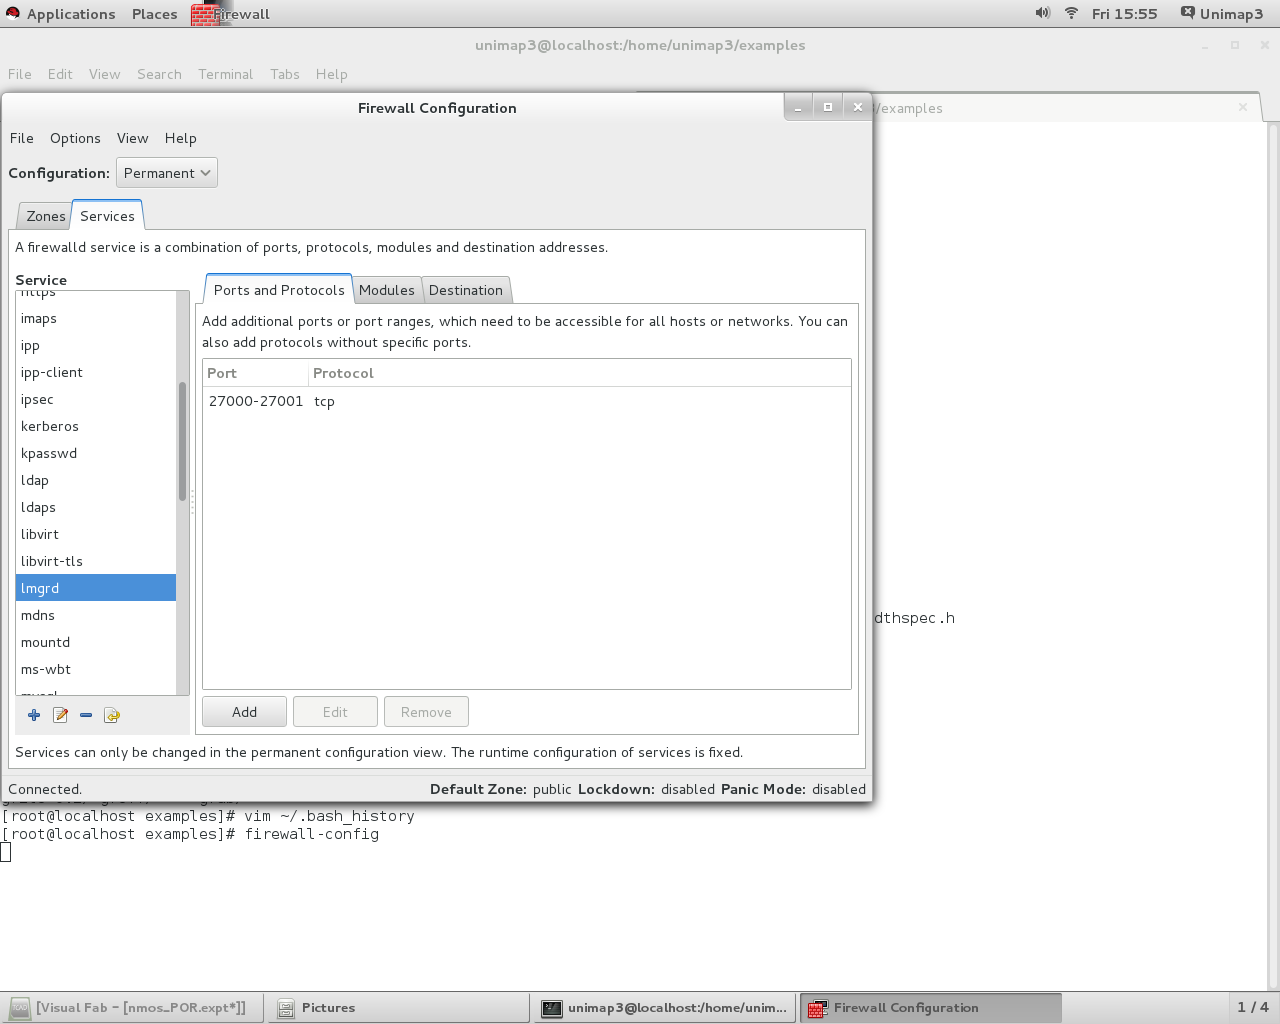
\includegraphics[width=0.8\textwidth]{plot/fw_service}\caption{In firewall configuration, add the lmgrd service.\label{fig:fw:service}}
\end{figure}



\subsubsection{Allow Access to FlexLM Service}

As shown in \ref{fig:fw:zone}, select the \guimenu{Zones} tab, check
the service \userinput{lmgrd} in the following zones:
\begin{itemize}
\item dmz
\item external
\item home
\item internal
\item public
\item trusted
\item work
\end{itemize}
\begin{figure}
\centering{}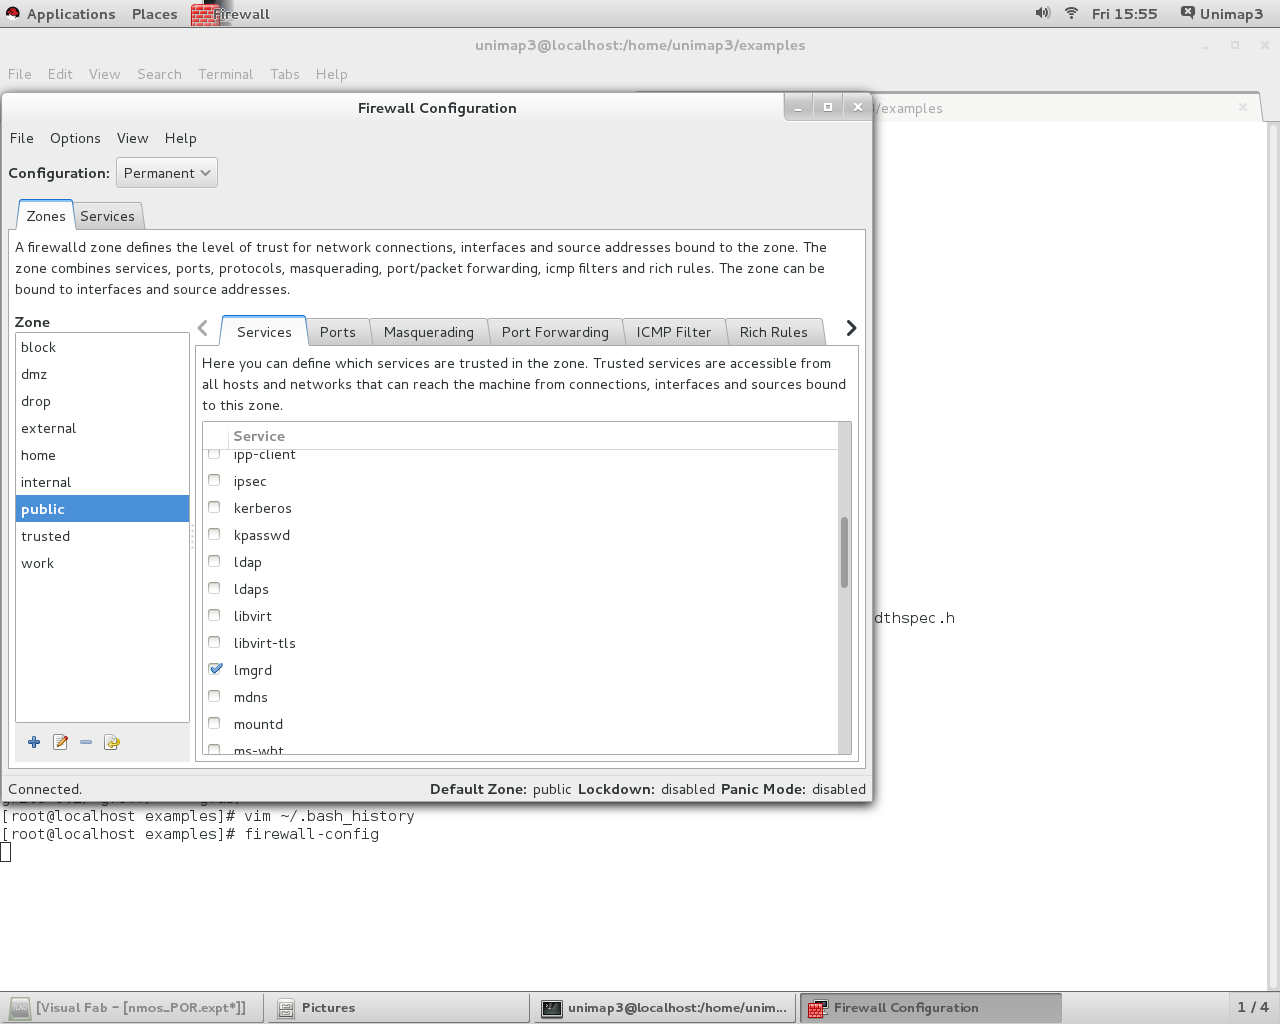
\includegraphics[width=0.8\textwidth]{plot/fw_zone}\caption{In firewall configuration, enable lmgrd service in zones.\label{fig:fw:zone}}
\end{figure}



\subsection{User Bash Profile}

Edit the file \filename{\$HOME/.bashrc}, append the following two
lines to the end of that file.

\begin{lstlisting}
export LM_LICENSE_FILE=27000@192.168.123.3
source /opt/cogenda/current/bin/setenv.sh
\end{lstlisting}


Note the IP address in this file. It is the IP address of the license
server. If the network setup changes, one has to update this IP address
on every workstation.

If there are more than one user accounts on this computer that will
use Cogenda software, repeat this procedure in each user's home directory.

After this, one can start the \command{VisualTCAD} or \command{VisualFab}
program to test the installation.
\end{document}
